\hypertarget{ht__resize_8c}{
\section{ht\_\-resize.c File Reference}
\label{ht__resize_8c}\index{ht_resize.c@{ht\_\-resize.c}}
}


\subsection{Detailed Description}
\begin{Desc}
\item[For internal use only.]
This file contains the implementation of the \hyperlink{group__dbprim__hash_ga16}{ht\_\-resize()} function, used to hint to the library that the hash table may perform better with a specific starting size.\end{Desc}


Definition in file \hyperlink{ht__resize_8c-source}{ht\_\-resize.c}.

{\tt \#include $<$stdlib.h$>$}\par
{\tt \#include $<$errno.h$>$}\par
{\tt \#include \char`\"{}dbprim.h\char`\"{}}\par
{\tt \#include \char`\"{}dbprim\_\-int.h\char`\"{}}\par


Include dependency graph for ht\_\-resize.c:\begin{figure}[H]
\begin{center}
\leavevmode
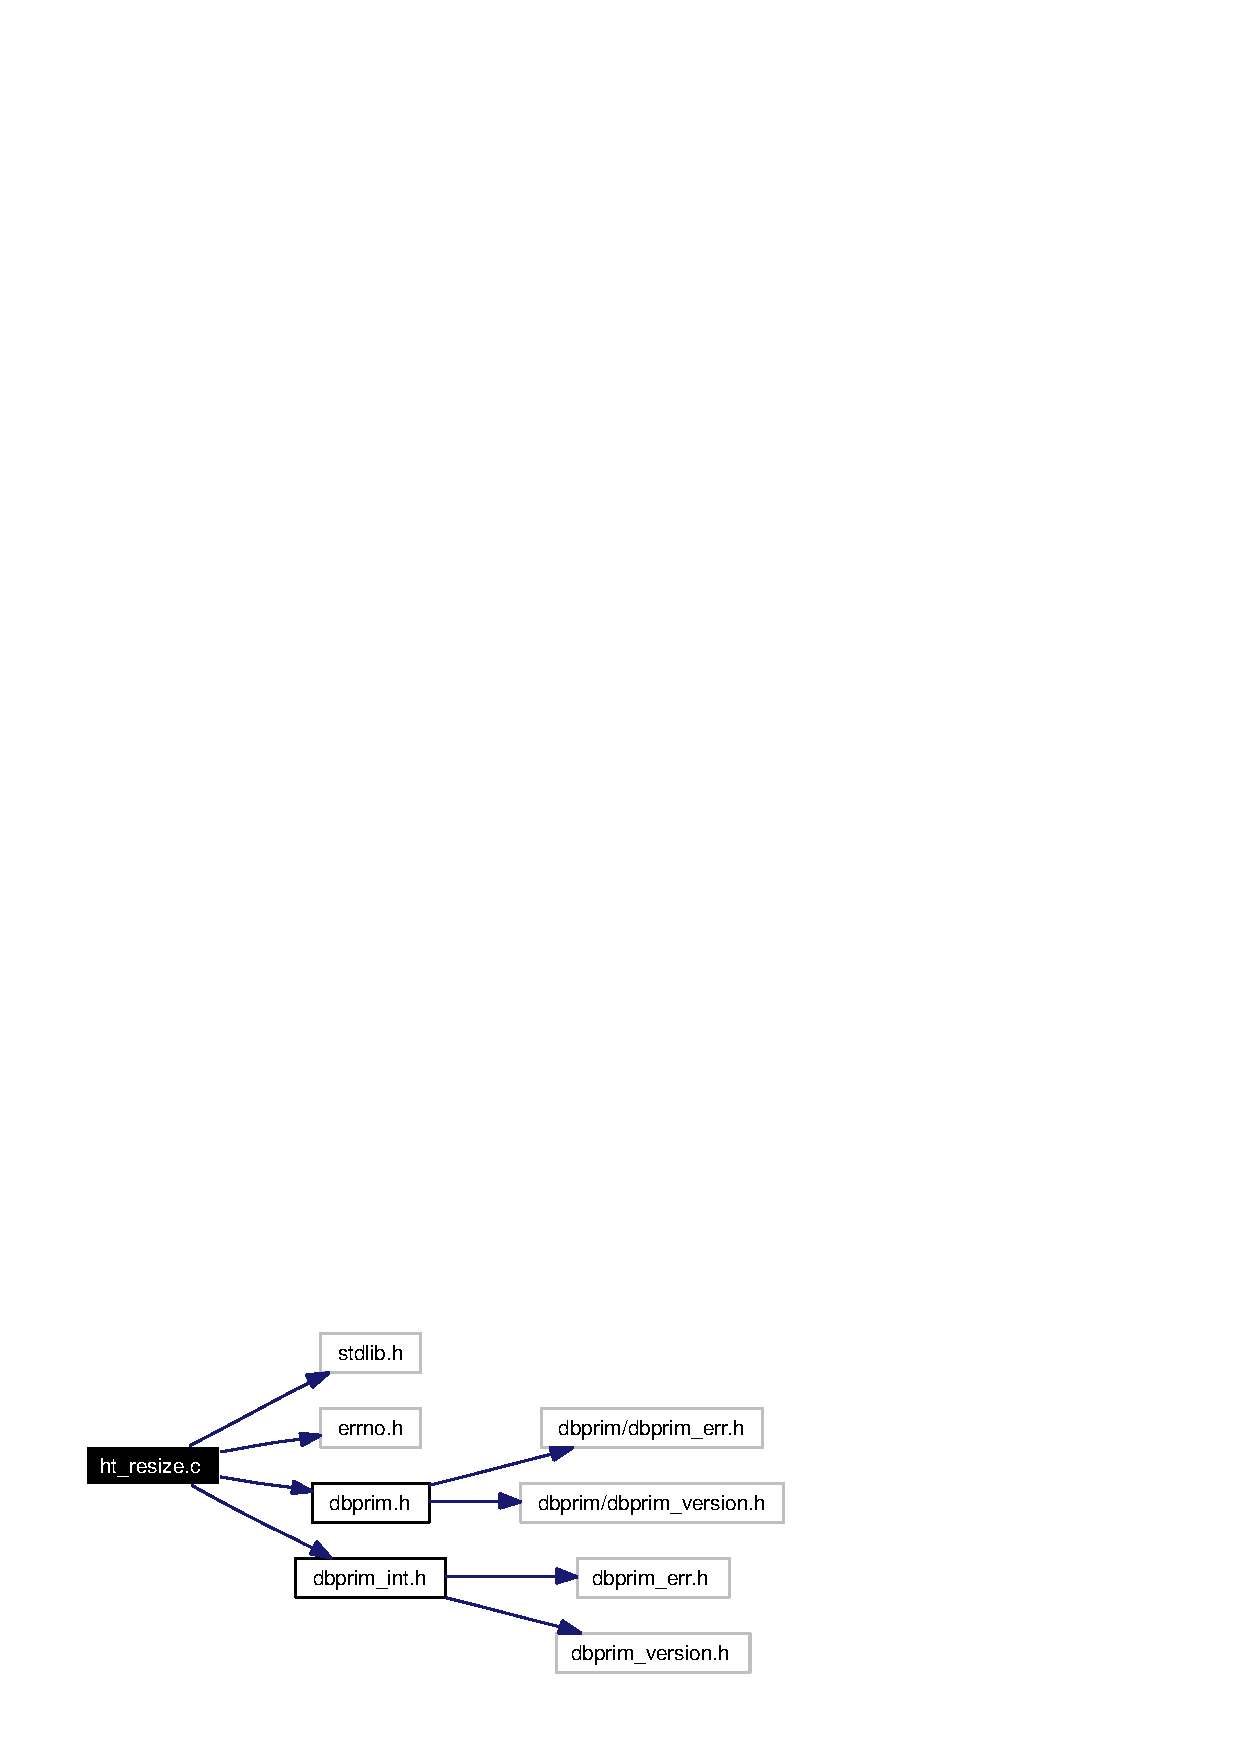
\includegraphics[width=190pt]{ht__resize_8c__incl}
\end{center}
\end{figure}
\subsection*{Functions}
\begin{CompactItemize}
\item 
unsigned long \hyperlink{group__dbprim__hash_ga16}{ht\_\-resize} (\hyperlink{struct__hash__table__s}{hash\_\-table\_\-t} $\ast$table, unsigned long new\_\-size)
\begin{CompactList}\small\item\em Resize a hash table. \item\end{CompactList}\end{CompactItemize}
